\phantomsection
\chapter{Facial expression recognition}

\noindent After having stated the conditions and motivations of this project, we will now describe the general structure a a facial expression recognition system. It can indeed be roughly summed up as classification applied to a pre-processed image.An overview of pre-processing steps will be done in this chapter, while feature extraction and classification will be more detailed respectively in Parts ~\ref{chap:extraction} and ~\ref{chap:classification}. Following sections will be about issues raised by facial expression recognition systems, and key requirements these systems have to meet in order to be considered acceptable.

\section{General structure}

\vspace{\baselineskip}
\noindent Facial expression recognition is a system enabling an automatic recognition of emotions displayed by a human face. Facial expression recognition can be image or video-based; it can also be computed in real-time if needed. Researchers usually try to recognize emotions out of static images. It can also be achieved real-time on video streams: While the person displays his/her emotions, the facial expression recognition system analyses the video, and detect the displayed emotion.
\newline

\noindent In both cases, facial expression recognition process is structured as in Figure~\ref{facial_expression_recognition_process}
\newline

\begin{figure}[!h]
\begin{center}
\noindent 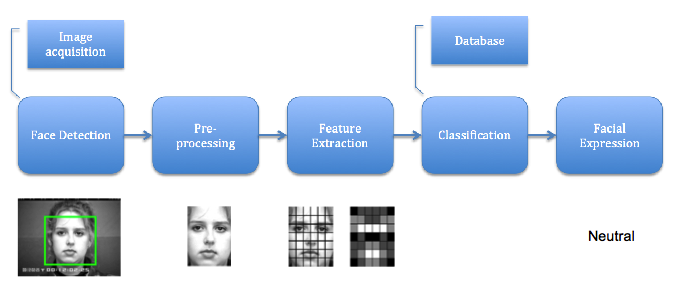
\includegraphics[scale=0.6]{figures/facial_expression_recognition_process} 
\newline
\caption{Facial expression recognition process}
\label{facial_expression_recognition_process}
\end{center} 
\end{figure}

\subsection{Image Acquisition}

\vspace{\baselineskip}
\noindent The first step is "Image Acquisition". Images used for facial expression recognition can be static images or image sequences, with the latter giving more informations about the displayed expression, i.e steps in muscles movement. About static images, facial expression recognition systems usually take 2D greyscale images as inputs. We can however expect future systems to use color images; first because of the increasing affordability of technologies and devices capable of capturing images or image sequences; then because colors can give more information on emotions, for example blushing \cite{CHI03}.
\newline

\subsection{Face Detection}

\vspace{\baselineskip}
\noindent Second step is "Face Detection". Indeed, in a static image and even more in an images sequence, this is an obvious need. Once the face has been detected, all other non-relevant information can be deleted. This step could hence be included in the next step, which is "Pre-processing", but because of its importance it can be considered as a step in itself. If working with image sequences or video streams, the face has to be detected and tracked. One of the most used and famous detection and tracking algorithm is the Viola-Jones algorithm, which will be explained further in Chapter~\ref{chap:vj}. This algorithm can be trained to detect all kind of objects, but is mostly used for face detection.
\newline

\subsection{Pre-processing}

\vspace{\baselineskip}
\noindent Third step is "Pre-processing", where image processing algorithms are applied to the image in order to prepare it for the next step. Pre-processing is usually about noise removal, normalization against the variation of pixel position or brightness, segmentation, location or tracking of parts of the face. Transformation, scaling and rotation of the head in the image or image sequence have an effect on emotion recognition. In order to solve this problem, the image can be geometrically standardized, with the eyes generally used as reference points \cite{CHI03}.
\newline

\subsection{Feature Extraction}

\vspace{\baselineskip}
\noindent Once the image has gone through the "Pre-processing" step, the next one is "Feature Extraction". In this step, data is converted "into a higher representation of shape, motion, color, texture, and spatial configuration of the face or its components" \cite{CHI03}. One of the main goals of this step is to reduce the dimensionality of the input data. The reduction procedure should retain "essential information possessing high discrimination power and high stability" \cite{CHI03}. There are a lot of features extraction methods. The most famous are : Principal Component Analysis (PCA), Linear Discriminant Analysis (LDA), Local Binary Patterns (LBP), Hidden Markov Models (HMM), Eigenfaces, Gabor Wavelets. This step will be detailed further in Part ~\ref{chap:extraction}. The extracted data is then used in the "Classification" step.
\newline

\subsection{Classification}

\noindent The classification step is the culminating point of the facial expression recognition process. There are many kinds of classification algorithms, some of them can even be used in the feature extraction part, as it will be detailed in Part ~\ref{chap:extraction}. This step takes into input a model previously trained with pre-processed data, and test data made of feature vectors extracted from the image we want to label. Feature vectors from pre-processed data and test data have to be obtained using the same feature extraction algorithm. The chosen classifier then outputs a value corresponding to the label of the class the picture belongs to.
%\vspace{\baselineskip}

\phantomsection
\section{Environment Setup}

\vspace{\baselineskip}
\noindent Our system will use the camera embedded into a Microsoft Kinect to record the user's video input. We will consider a casual use of the camera, the user sitting in front of the computer, the camera being next to it, as seen in \textbf{\color{red} Insert picture of the setting \& ref to figure}. This camera provides a 640$\times$480 pixels frame resolution, while recording at 30 FPS.
\newline

\noindent For development and training purposes we will use some pre-existing emotion datasets, in order to validate the efficiency of the system before testing it in real conditions.
\newline

\phantomsection
\section{Facial Expression Datasets}

\vspace{\baselineskip}
\noindent Databases are very important for facial expression recognition system.
\newline

\noindent Using the same databases as in previous studies allows performance and accuracy comparisons between new implementations and previously obtained results. Since most studies draw their results on the same databases, it is then relatively easy to compare them and choose a database suitable for our system.
\newline

\noindent Databases are however difficult to build. Indeed, it has to be obtained following a meticulous procedure while being exhaustive so it can be considered as representative. The majority of actual databases use posed expressions rather than spontaneous ones, this choice having a major influence on facial expression recognition systems. This explains why some databases are updated, and now integrate spontaneous expressions. Even with this transition from posed expressions to spontaneous expressions, there are other requirements that should be met to have a standardized database.Its content should be of different resolutions and scales, and should also contain exposition under different conditions, i.e changes in lightning, occlusions or different head angles \cite{BET12}.  
\newline

\noindent Constructing a database is then a tedious task because of all these requirements to meet. Consequently, most studies are based on already existing datasets. The 3 datasets described afterwards are popular and freely available facial expression datasets which have been used a numerous amount of times in the past few years. Our system will then be trained and tested with one or several of these databases.
\newline

\subsection{Japanese Female Facial Expression Database (JAFFE)}

\vspace{\baselineskip}
\noindent This database contains 213 images of 7 facial expressions (6 basic facial expressions: happy, angry, afraid, disgusted, sad, surprised, and 1 neutral facial expression). Each expression has been photographed three or four times. Each image has been rated on 6 emotion adjectives by 60 Japanese subjects. All images come from 10 Japanese female models.  The database was planned and assembled by Miyuki Kamachi, Michael Lyons, and Jiro Gyoba \cite{JAFFE}.
\newline

\noindent This database contains only posed expressions. The photos have been taken under strict  and controlled conditions: similar lighting and hair tied so there is no facial occlusion \cite{BET12}. 
\newline

\noindent An example of images contained in the database is given by Figure~\ref{jaffe_7facialexpressions}. In this figure, this is a female subject displaying 7 different emotional expressions (neutral, happy, angry, afraid, disgusted, sad, surprised). 
\newline

\begin{figure}[!h]
\begin{center}
\noindent 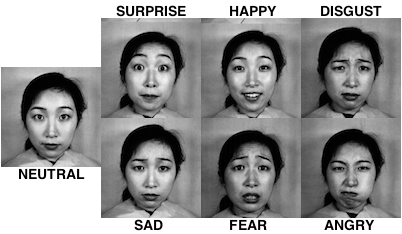
\includegraphics[scale=0.75]{figures/jaffe_7facialexpressions} 
\newline
\caption{Example of images from JAFFE database}
\label{jaffe_7facialexpressions}
\end{center} 
\end{figure}

\subsection{Karolinska Directed Emotional Faces Database (KDEF)}

\vspace{\baselineskip}
\noindent The Karolinska Directed Emotional Faces (KDEF) contains 4900 pictures of human facial expressions. The material was developed in 1998 by Daniel Lundqvist, Anders Flykt and Professor Arne Ohman at Karolinska Institutet, Department of Clinical Neuroscience, Section of Psychology, Stockholm, Sweden \cite{KDEF}.
\newline

\noindent The database was first developed for psychological and medical research purposes. It was created so it could used in perception, attention, emotion, memory and backward masking experiments. This database has also been built under controlled conditions. Indeed, researchers tried to maintain constant and soft lighting for each subject. Furthermore, they made their subjects wear the same grey T-shirts, and used a grid to center the participants faces while they were shot. This grid was also used to place eyes and mouths at the same position in fixed image coordinates during scanning \cite{KDEF}.
\newline

\noindent The database contains 70 individuals (35 males and 35 females), from 20 to 30 years, each one displaying 7 different emotional expressions (neutral, happy, angry, afraid, disgusted, sad, surprised). Each expression has been photographed (twice) from 5 different angles (-90, -45, 0, +45, +90 degrees: i.e. full left profile, half left profile, straight, half right profile, full right profile)  \cite{KDEF}.
\newline

\noindent An example of images contained in the database is given in Figure~\ref{kdef_7facialexpressions}which represents a female subject photographed from a straight angle and displaying 7 different emotional expressions (neutral, happy, angry, afraid, disgusted, sad, surprised).
\newline

\begin{figure}[!h]
\begin{center}
\noindent 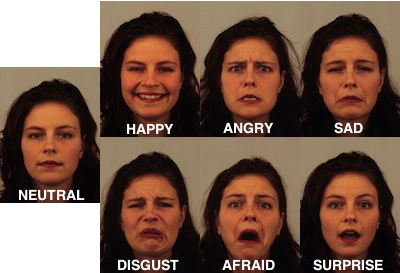
\includegraphics[scale=0.65]{figures/kdef_7facialexpressions} 
\newline
\caption{Example of images from KDEF database}
\label{kdef_7facialexpressions}
\end{center} 
\end{figure}

\subsection{Montreal Set of Facial Displays of Emotion Database (MSFDE)}

\vspace{\baselineskip}
\noindent This database contains facial expressions of European, Asian, and African subjects, from both genders. Each expression was created by directly asking the subject to express this emotion \cite{MSFDE}.
\newline

\noindent The database contains expressions of happiness, sadness, anger, fear, disgust, and embarrassment, along with a neutral facial expression. All expressions have been photographed at 5 different levels of intensity \cite{MSFDE}.
\newline

\noindent An example of images contained in the database is given in Figure~\ref{msfde_7facialexpressions}, where an African female subject displays 7 different emotional expressions (neutral, happy, angry, afraid, disgusted, sad, ashamed).
\newline

\begin{figure}[!h]
\begin{center}
\noindent 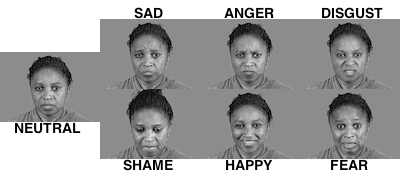
\includegraphics[scale=0.8]{figures/msfde_7facialexpressions} 
\newline
\caption{Example of images from MSDFE database}
\label{msfde_7facialexpressions}
\end{center} 
\end{figure}

\phantomsection
\section{Issues}

\vspace{\baselineskip}
\subsection{Datasets}

\vspace{\baselineskip}
\noindent Databases can be a source of issues. As said previously, databases should meet a number of requirements in order to be as exhaustive and efficient as possible. 
\newline

\noindent In order to build a facial expression recognition system efficient in live conditions,, it should be able to recognize spontaneous expressions rather than posed expressions. Indeed, spontaneous expressions are closer to reality than posed expressions, the latter being exaggerated to facilitate their labelling and recognition. While creating a database of spontaneous expressions, Sebe and al \cite{SEB07} made some observations of the major problems they encountered \cite{BET12}:
\newline
\begin{itemize}
  \item The same emotions can be expressed at different intensities by different subjects;
  \item As soon as the subject is aware of being photographed and studied, the authenticity of the emotion is lost;
  \item Because of the laboratory conditions, even if the subject is not aware of being photographed or recorded, the subject is not encouraged to display spontaneous expressions.
\end{itemize}

\vspace{\baselineskip}
\noindent In order to overcome these problems, they came up with a method. Their solution was to record facial expressions with a camera hidden in a video kiosk displaying emotion inducing videos. Subjects were notified of the recording after it was done, and were asked a permission to use recorded sequences for research studies. The subjects then explained which emotions they felt and expressed, their replies being documented even if it did not match the recorded expressions \cite{SEB07}.
\newline

\noindent The researches found that a wide range of expressions are hard to induce, particularly fear and sadness. They also found that spontaneous expressions could be misleading: some subjects express one emotion while feeling another one (for example, one subject was showing sadness while being happy) \cite{SEB07}.
\newline

\noindent In a nutshell, databases bring some issues that can affect the authenticity of the recognition system. It depends of the type of expressions: spontaneous or posed expressions. If the system aims to recognize facial expressions of people unaware of it, spontaneous expressions databases will be used but, as seen previously, it can lead to authenticity issues. If the system aims to recognize facial expressions of people asked to express certain emotion, posed expressions databases will be used, but the result will not be close to reality.
\newline

\subsection{Real-time}

\vspace{\baselineskip}
\noindent The primary goal of the facial expression recognition system described in this paper is to perform real-time facial expression recognition. As a real-time application, the processing time should be taken into account. Indeed, if it is too long, the system will not be responsive enough to be labelled as real-time.
\newline

\noindent This is one of the challenges of this kind of system, because processing is usually really heavy no matter which algorithm is used. Most facial expression recognition applications should be working in real-time conditions, for example in robotics or in surveillance. A solution could be to find new algorithms for facial expression recognition or to improve and lighten already existing algorithms.
\newline

\subsection{Conditions}

\vspace{\baselineskip}
\noindent Another one of the challenges of this kind of system is to be independent of recording conditions. It means that the recognition should not be disturbed for example by occlusions, or difference in the lighting, or even by the angle between the face and the camera. These examples cover almost all conditions that can change during the recording, and have an influence on the recognition system. 
\newline

\subsubsection{Occlusion}

\vspace{\baselineskip}
\noindent "Occlusion" defines all elements covering the face, partly or entirely. For example, a beard, a scarf masking the bottom of the face, glasses or bangs. By hiding a part of the face, these occlusions can affect the recognition. Indeed, facial expression recognition systems are based on comparison of features, and if all the features cannot be compared because something is covering a part of the face, the recognition accuracy is affected. In order to compensate for this problem, some databases includes data with occluded faces, for example with beards, glasses or scarves. This is the case for the AR Face database. Some examples of images contained in this database are given by Figures~\ref{arface_example2} and ~\ref{arface_example3} \cite{ARFACE}.
\newline

\begin{figure}[!h]
\begin{center}
\noindent 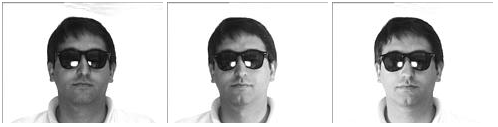
\includegraphics[scale=0.7]{figures/arface_example2} 
\newline
\caption{Example eye occlusion in the AR Face database}
\label{arface_example2}
\end{center} 
\end{figure}

\begin{figure}[!h]
\begin{center}
\noindent 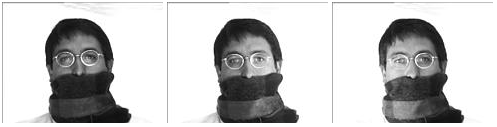
\includegraphics[scale=0.7]{figures/arface_example3} 
\newline
\caption{Example of face occlusion in the AR Face database}
\label{arface_example3}
\end{center} 
\end{figure} 

\subsubsection{Lighting}

\vspace{\baselineskip}
\noindent As for occlusion, lighting is an element that can affect recognition effectiveness. With different lighting conditions from those in the database, recognition will be less efficient. All conditions different from those recorded  in the database on which the recognition process is based will impact the system. If images are brighter or darker than reference data, some details can disappear, or some features will not be recognized as well as if the conditions were identical. In order to compensate for this problem, databases can include data with different lighting conditions. This is the case for the AR Face database and an example of the images contained in this database is given by Figure~\ref{arface_example1} \cite{ARFACE}:
\newline

\begin{figure}[!h]
\begin{center}
\noindent 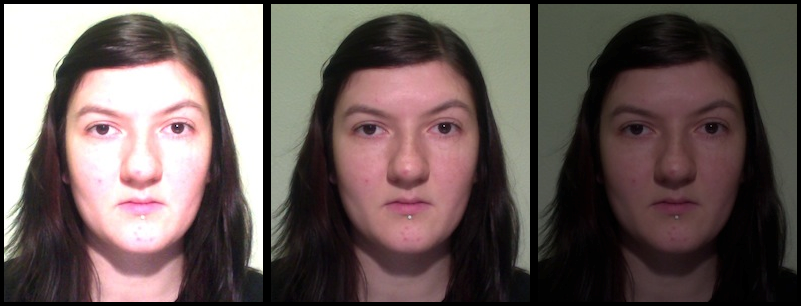
\includegraphics[scale=0.7]{figures/arface_example1} 
\newline
\caption{Example of different lighting conditions (from left to right: dark to bright) in the AR Face database}
\label{arface_example1}
\end{center} 
\end{figure}

\subsubsection{Angle}

\vspace{\baselineskip}
\noindent Head angle is one of the most impacting conditions during recognition. Indeed, some features can be occluded or disappear if the head does not properly face the camera. This issue also rises if the system is not tuned to work with head angles other than straight profile. For example, with a profile angle, one eye, half of the nose and of the mouth disappear. If the database does not contain samples with profile faces, the recognition will fail. However, if the database contains images from straight angle as well as from different profile angles, recognition will be possible. An example of different images taken from different angles for one emotion, "Fear", from the KDEF database is given in Figure~\ref{kdef_example_angle}:
\newline

\begin{figure}[!h]
\begin{center}
\noindent 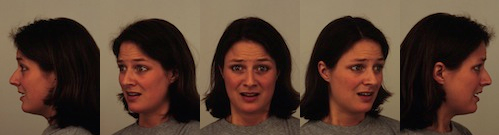
\includegraphics[scale=0.8]{figures/kdef_example_angle} 
\newline
\caption{Example of different angles for the "Fear" emotion (from left to right: full left profile, half left profile, straight, half right profile, full right profile) in the KDEF database}
\label{kdef_example_angle}
\end{center} 
\end{figure}

\phantomsection
\section{Requirements}

\vspace{\baselineskip}
\noindent Based on everything said previously, our facial expression recognition system can be defined by some requirements prior to its implementation. Additional requirements may be defined further. Here are the requirements already defined :
\newline

\begin{itemize}
  \item Able to recognize basic emotions : 
  \noindent As explained before, facial expression recognition systems are able to recognize 6 basic emotions and the neutral state. This system should be able to do the same: recognize the 6 basic emotion that are "Happiness", "Fear", "Surprise", "Disgust", "Sadness", "Anger" and the neutral state.
\newline

  \item Able to work in real-time : 
  \noindent This system should be able to recognize facial expressions in real-time. It means that it can recognize expressions based on video sequences. It also means that the algorithm for feature extraction has to be carefully optimized so it is able to compute facial features in a decent amount of time. 
\newline

  \item Recognition from straight angle of the face : 
  \noindent This system should be able to recognize facial expression from a straight angle of the face. It means that the system should be able to detect faces in front of the camera lens, and recognize expressions in these faces. It might not be able to recognize emotions on a face on a profile or half-profile angle.
\newline

  \item Recognition with no occlusion : 
  \noindent This system should be able to recognize emotions with no occlusion on the subject's face. It means that the face should not be covered in any way: no glasses, no beard or no scarf. The face should also be complete, not cut and not masked.
\newline

  \item Recognition with no changes in lighting : 
  \noindent This system should be able to recognize emotions under constant lighting conditions during the recognition process. Moreover, the intensity level of the light should be as close as possible to the one of the database. This way the lighting would not have any influence on the recognition process.
\newline
\end{itemize}











